\chapter{Application Development Plan}

A visualization for the plan for this project can be seen in the Gannt chart in Figure \ref{fig:gannt}.
\begin{figure}
	\caption[Gannt Chart of the Project]{Gannt chart showing the project's planned process over the academic year.}
	\label{fig:gannt}
	\begin{center}
	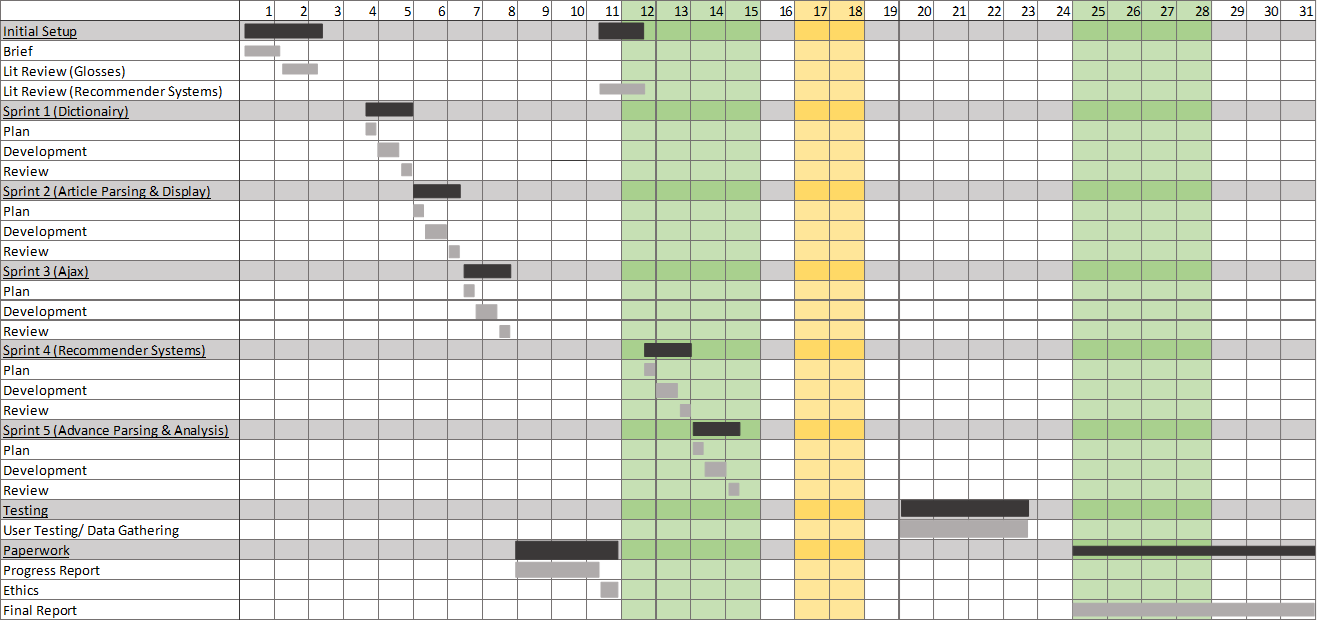
\includegraphics[width=\textwidth]{Graphics/Gannt}
	\end{center}
\end{figure} 

\section{Background Reading}

The plan details that reading was divided into two parts, reading about glosses and reading about difficulty rating systems. Reading about glosses was performed at the start of the project. Later, once the gloss section of the application had been developed, reading about difficulty rating systems was done. The reading was done this way as the difficulty rating system was not part of the minimum viable project, so the reading about it could be left until after the development of the minimum viable project was complete. The vast majority of this reading was academic, looking into the effectiveness of various glosses and methods of rating the difficulty of articles.

Other reading was done during the planning stage of each sprint, this reading was more technical and was about researching and deciding upon the technologies that were to be used for that sprint. Once a technology had been decided upon, there was some time spent on learning how to integrate it with project.


\section{Development}

The application was developed using AGILE methods. These methods were used as they allowed the developer to have regular meetings with the project supervisor, discussing the progress made, what was left to be done and whether or not it was achievable. These meetings meant that the functionality of the application was revised several times while still keeping to the outlines goals. 

\section{Testing}

Each sprint was tested during and at the end of its development to check both its performance and whether or not it integrated with the rest of the application. This testing was either unit testing or functional testing, depending on the sprint. This testing allowed to see whether or not the sprint was performing as expected.

Finally, user testing was done once all the sprints were completed. It involved users using the application to read three articles, and then filling out a feedback survey about their experiences with it. In addition, the users' use of the application was tracked, seeing what words they requested and what articles they read. Ethics approval for this test was obtained from the ECS ethics board. 